\documentclass[a4paper,titlepage,12pt]{article}
\usepackage[utf8]{inputenc} %Make sure all UTF8 characters work in the document
\usepackage{color}
\usepackage{graphicx}
\usepackage{titling}
\usepackage{tabularx}
\usepackage{longtable}
\usepackage[yyyymmdd]{datetime}
\usepackage[figurename=Figur]{caption}
\usepackage{pbox}
\usepackage{booktabs}

%Set page size
\usepackage{geometry}
\geometry{margin=3cm}

\renewcommand{\dateseparator}{-}
\renewcommand{\contentsname}{Innehållsförteckning}

%%%%%%%%%%%%%%%%%%%%%%%%%%%%%%%
% Header and footer
%%%%%%%%%%%%%%%%%%%%%%%%%%%%%%%
\usepackage{fancyhdr}
\pagestyle{fancy}

\lhead{
\includegraphics[width=0.15\linewidth]{../images/logo_full.png}}
\chead{Systemskiss för sexbent robot}
\rhead{\today}
\setlength\headheight{26pt} 

\lfoot{TSEA29 --- KMM \\ LIPS Systemskiss}
\rfoot{Grupp 9 \\ LiTHe Hex}

\pretitle{%
    \begin{center}
        \LARGE
        
\includegraphics[width=6cm]{../images/logo_full.png}\\[\bigskipamount]
}

\posttitle{\end{center}}

\begin{document}
    \title{\LARGE
        \textbf{Systemskiss för sexbent robot} \\
        \vspace*{0.5\baselineskip}
        \large
        Redaktör Frans Skarman \\
        Grupp 9 \\
        \small
        \vspace*{0.5\baselineskip}
        Version 0.1}

    \date{\today}

	\maketitle
	
	\newpage
	
	\begin{center}

		%%%%%%%%%%%%%%%%%%%%%%%%%%%%%%%%%%%%%%%%%%%%%%%%%%%%%%%%%%%%%%%%%%%%%%%%%%%%%%%%%
		%						Medlemmar
		%%%%%%%%%%%%%%%%%%%%%%%%%%%%%%%%%%%%%%%%%%%%%%%%%%%%%%%%%%%%%%%%%%%%%%%%%%%%%%%%%

		\section*{Projektidentitet}
		Grupp 9, Ht 2016, LiTHe Hex

		Linköpings Tekniska Högskola, ISY

		\begin{table}[h]
			\begin{center}
				\begin{tabular}[pos]{ l l l }
					\textbf{Namn} & \textbf{Ansvar} & \textbf{E-post} \\ \midrule
					Emil Segerbäck & Webbgränssnitt & emise935@student.liu.se \\ \midrule
					Frans Skarman & Dokumentansvarig & frask812@student.liu.se \\ \midrule
					Hannes Tuhkala & & hantu447@student.liu.se \\ \midrule
					Malcolm Vigren & Projektledare & malvi108@student.liu.se \\ \midrule
					Noak Ringman &  & noari093@student.liu.se \\ \midrule
					Olav Övrebö &  & olaov121@student.liu.se \\ \midrule
					Robin Sliwa &  & robsl733@student.liu.se \\
				\end{tabular}
			\end{center}
		\end{table}

		\centering
		\textbf{Kursansvarig}: Tomas Svensson Rum 3B:528 013--28 13 68 tomas.svensson@liu.se

		\newpage
		\tableofcontents
		\newpage


		%%%%%%%%%%%%%%%%%%%%%%%%%%%%%%%%%%%%%%%%%%%%%%%%%%%%%%%%%%%%%%%%%%%%%%%%%%%%%%%%%
		%						Historik
		%%%%%%%%%%%%%%%%%%%%%%%%%%%%%%%%%%%%%%%%%%%%%%%%%%%%%%%%%%%%%%%%%%%%%%%%%%%%%%%%%

		\section*{Dokumenthistorik}
		\begin{table}[h]
			\begin{tabular}[pos]{ l l l l l }
				\textbf{Version} & \textbf{Datum} & \textbf{Utförda förändringar} 
				& \textbf{Utförda av} & \textbf{Granskad} \\ \midrule

				0.1 & 2016--09--09 & Första utkastet & Projektgruppen & \\

			\end{tabular}
		\end{table}
	\end{center}

	%%%%%%%%%%%%%%%%%%%%%%%%%%%%%%%%%%%%%%%%%%%%%%%%%%%%%%%%%%%%%%%%%%%%%%%%%%%%%%%%%
	%						Inledning
	%%%%%%%%%%%%%%%%%%%%%%%%%%%%%%%%%%%%%%%%%%%%%%%%%%%%%%%%%%%%%%%%%%%%%%%%%%%%%%%%%

	\newpage

	\section{Inledning}
	I detta dokument beskrivs funktionaliteten produkten ska ha vid leverans.
    All funktionalitet har strukturerats i olika krav där det blir tydligt om
    kravet är uppfyllt eller inte. Krav har olika nivåer där nivå 1 är ska-krav
    som måste ha uppfyllts vid leverans. Nivå 2 ses som bör-krav och uppfylls i
    mån av tid.

	%%%%%%%%%%%%%%%%%%%%%%%%%%%%%%%%%%%%%%%%%%%%%%%%%%%%%%%%%%%%%%%%%%%%%%%%%%%%%%%%%
	%						Översikt
	%%%%%%%%%%%%%%%%%%%%%%%%%%%%%%%%%%%%%%%%%%%%%%%%%%%%%%%%%%%%%%%%%%%%%%%%%%%%%%%%%

  \newpage
	\section{Systemöversikt}
	Systemet ska innehålla tre enheter. En centralenhet för kommunikation med en
    dator, en motorikenhet som sköter hur benen rör sig samt en sensorenhet som
    tolkar sensordata. Centralenheten är även den enhet som tar beslut och
    kommunicerar med de andra enheterna. Se Figur. 1 för en översiktsbild av
    systemet.
	\begin{figure}[h]
		\centering
		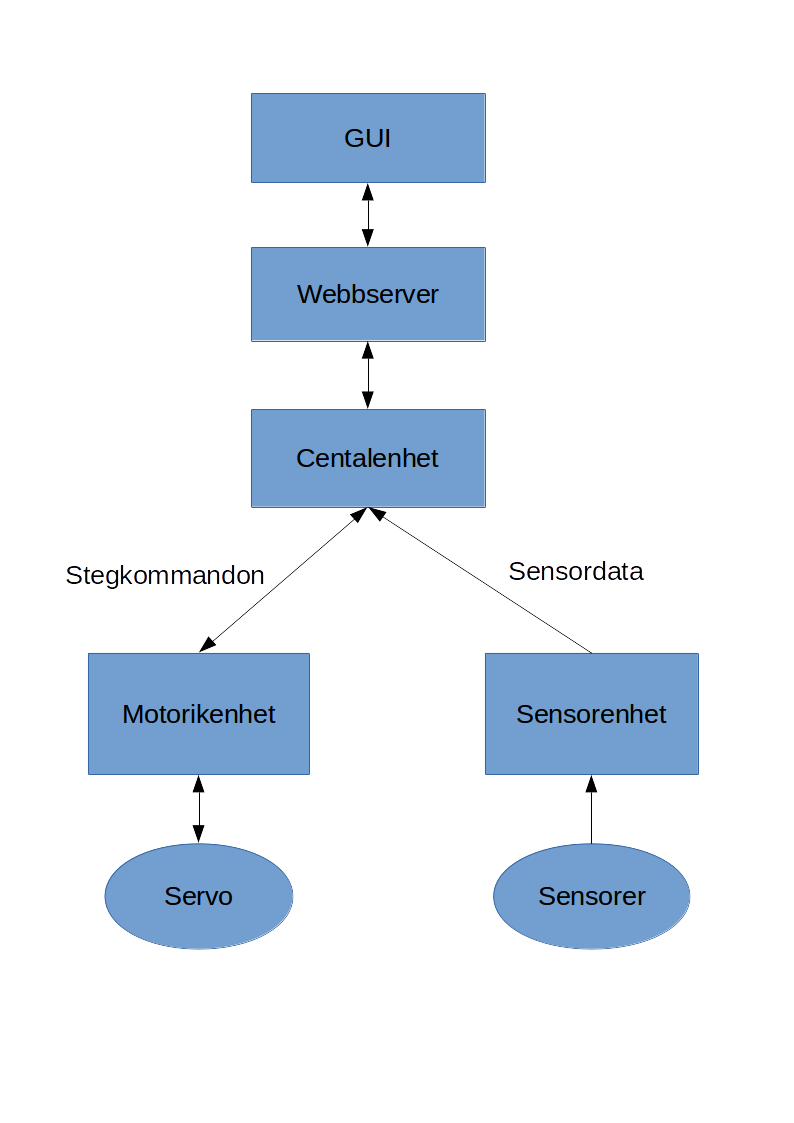
\includegraphics[width=0.5\linewidth]{../images/overview.png}
		\caption{Översikt av systemet\label{fig:overview}}
	\end{figure}

	\subsection{Kommunikation mellan enheterna}
	Kommunikation kan ske med UART, SPI eller I2C. AVR-processorerna har
	2 UART-, 3 SPI- och en I2C-ingång medan Raspberry PIen har 1 UART-, 2 SPI- och
	en I2C-ingång. 

	\subsubsection{Förslag 1}
	Om vi vill ha en LIDAR-avståndsmätare kommer sensorenhetens I2C-port att gå åt
	till kommunikation med avståndsmätaren. Sensorenheten måste alltså kommunicera med
	centralenheten med UART eller SPI.

	

	\subsection{Grov beskrivning av systemet}
	Här var det text här var det text här var det text
	här var det text här var det text här var det text
	här var det text här var det text här var det text.
	
	
	\subsection{Ingående delsystem}
	Här var det text här var det text här var det text
	här var det text här var det text här var det text
	här var det text här var det text här var det text.
	
	
	\section{Centralenheten}
	Centralenheten har 4 huvudsyften: navigation/beslutsfattning, hinderdetektion samt
	kommunikation med omvärlden.

	\subsection{Navigation och beslutsfattning}

	\subsection{Hinderdetektion}

	\subsection{Kommunikation}



	%%%%%%%%%%%%%%%%%%%%%%%%%%%%%%%%%%%%%%%%%%%%%%%%%%%%%%%%%%%%%%%%%%%%%%%%%%%%%%%%%
	%						Motorikenheten
	%%%%%%%%%%%%%%%%%%%%%%%%%%%%%%%%%%%%%%%%%%%%%%%%%%%%%%%%%%%%%%%%%%%%%%%%%%%%%%%%%
	
	\section{Motorikenheten}
    Motorikenheten översätter signaler från centralenheten, angeende önskad förflyttning, 
    till instruktioner för benens förflyttning, och förser centralenheten med data om
    benens motstånd.
    
    	\subsection{Alternativ 1: Anpassad gångstil}
    Motorikenheten mottar instruktioner från centralenheten, angeende önskad hastighet, 
    rotation och riktning för förflyttnnig. Den behandlar detta och räknar ut en lämplig 
    gångstil, och signalerar nödvändiga vinklar till de sex benen. 
    
    	\subsubsection{Planläggning}
    Första steget i motorikenheten för en anpassad gångstil är att utifrån efterfrågad
    förflyttning avgöra en önskad slutposition för respektive ben, som för roboten närmre 
    ett läge angivet av centralenheten. Utifrån hastighet kan förflyttningsvektorerna 
    från nuvarande läge för nuvarande ben skalas ner eller upp, inom rimligheten för vad
    benen kan nå. För flyttning sker för vänster fram- och bak-ben och höger 
    mittben, eller för höger fram- och bak-ben och vänster mittben, alternerande för varje
    förflyttningscykel. När ett sett förflyttas, skiftas de markfästa benen vid behov för 
    att flytta själva kroppen. 
    
    	\subsubsection{Invers kinematik}
    Andra steget i motorikenheten för en anpassad gångstil är beräkning av benens vinklar;
    utifrån kända längder på benen  och önskad vågrät vinkel och längd till slutposition 
    används trigonometri för att avgöra slutgiltiga aktuatorvinklar.
    
    	\subsection{Alternativ 2: Hårdkodad}
    Motorikenheten förses med en uppsättning hårdkodade instruktioner för benrörelser, och
    väljer bland dessa utifrån försedda indata. Hårdkodade rörelser inkluderar rotation på 
    plats, rörelse framåt (två hastigheter), bakåt och i sidled, rörelse med svag rotation, 
    bestigning av hinder (i mån av uppfyllande av detta sekundära krav). 
    
    	\subsection{Alternativ 3: Att skrivas}
    
	%%%%%%%%%%%%%%%%%%%%%%%%%%%%%%%%%%%%%%%%%%%%%%%%%%%%%%%%%%%%%%%%%%%%%%%%%%%%%%%%%
	%						Sensorenheten
	%%%%%%%%%%%%%%%%%%%%%%%%%%%%%%%%%%%%%%%%%%%%%%%%%%%%%%%%%%%%%%%%%%%%%%%%%%%%%%%%%
	\section{Sensorenheten}
    
    Sensorenheten är den enhet som ger roboten sinnen för omvärlden, så att den
    kan navigera autonomt 

    \subsection{Styrenhet}

    \subsection{Gyro}
    
    \subsection{Avståndssensorer i sidled}


\end{document}
